% This is "sig-alternate.tex" V2.1 April 2013
% This file should be compiled with V2.5 of "sig-alternate.cls" May 2012
%
% This example file demonstrates the use of the 'sig-alternate.cls'
% V2.5 LaTeX2e document class file. It is for those submitting
% articles to ACM Conference Proceedings WHO DO NOT WISH TO
% STRICTLY ADHERE TO THE SIGS (PUBS-BOARD-ENDORSED) STYLE.
% The 'sig-alternate.cls' file will produce a similar-looking,
% albeit, 'tighter' paper resulting in, invariably, fewer pages.
%
% ----------------------------------------------------------------------------------------------------------------
% This .tex file (and associated .cls V2.5) produces:
%       1) The Permission Statement
%       2) The Conference (location) Info information
%       3) The Copyright Line with ACM data
%       4) NO page numbers
%
% as against the acm_proc_article-sp.cls file which
% DOES NOT produce 1) thru' 3) above.
%
% Using 'sig-alternate.cls' you have control, however, from within
% the source .tex file, over both the CopyrightYear
% (defaulted to 200X) and the ACM Copyright Data
% (defaulted to X-XXXXX-XX-X/XX/XX).
% e.g.
% \CopyrightYear{2007} will cause 2007 to appear in the copyright line.
% \crdata{0-12345-67-8/90/12} will cause 0-12345-67-8/90/12 to appear in the copyright line.
%
% ---------------------------------------------------------------------------------------------------------------
% This .tex source is an example which *does* use
% the .bib file (from which the .bbl file % is produced).
% REMEMBER HOWEVER: After having produced the .bbl file,
% and prior to final submission, you *NEED* to 'insert'
% your .bbl file into your source .tex file so as to provide
% ONE 'self-contained' source file.
%
% ================= IF YOU HAVE QUESTIONS =======================
% Questions regarding the SIGS styles, SIGS policies and
% procedures, Conferences etc. should be sent to
% Adrienne Griscti (griscti@acm.org)
%
% Technical questions _only_ to
% Gerald Murray (murray@hq.acm.org)
% ===============================================================
%
% For tracking purposes - this is V2.0 - May 2012

\documentclass{sig-alternate-05-2015}
%\usepackage{subfig}



\begin{document}

%
% --- Author Metadata here ---
\setcopyright{acmlicensed}
\conferenceinfo{SUI '16,}{October 15--16, 2016, Tokyo, Japan.}
\isbn{978-1-4503-4068-7/16/10}
\acmPrice{\$15.00}
\doi{http://dx.doi.org/XXXX.XXXX}
% --- End of Author Metadata ---

\title{A Metric for Hand Comfort/Discomfort Evaluation} 
\subtitle{Towards Expressivity in Spatial Control}
%\titlenote{(Produces the permission block, and
%copyright information). For use with
%SIG-ALTERNATE.CLS. Supported by ACM.}}
%\subtitle{[Extended Abstract]
%\titlenote{A full version of this paper is available as
%\textit{Author's Guide to Preparing ACM SIG Proceedings Using
%\LaTeX$2_\epsilon$\ and BibTeX} at
%\texttt{www.acm.org/eaddress.htm}}}
%
% You need the command \numberofauthors to handle the 'placement
% and alignment' of the authors beneath the title.
%
% For aesthetic reasons, we recommend 'three authors at a time'
% i.e. three 'name/affiliation blocks' be placed beneath the title.
%
% NOTE: You are NOT restricted in how many 'rows' of
% "name/affiliations" may appear. We just ask that you restrict
% the number of 'columns' to three.
%
% Because of the available 'opening page real-estate'
% we ask you to refrain from putting more than six authors
% (two rows with three columns) beneath the article title.
% More than six makes the first-page appear very cluttered indeed.
%
% Use the \alignauthor commands to handle the names
% and affiliations for an 'aesthetic maximum' of six authors.
% Add names, affiliations, addresses for
% the seventh etc. author(s) as the argument for the
% \additionalauthors command.
% These 'additional authors' will be output/set for you
% without further effort on your part as the last section in
% the body of your article BEFORE References or any Appendices.




\numberofauthors{2} %  in this sample file, there are a *total*
% of EIGHT authors. SIX appear on the 'first-page' (for formatting
% reasons) and the remaining two appear in the \additionalauthors section.
%
\author{
% You can go ahead and credit any number of authors here,
% e.g. one 'row of three' or two rows (consisting of one row of three
% and a second row of one, two or three).
%
% The command \alignauthor (no curly braces needed) should
% precede each author name, affiliation/snail-mail address and
% e-mail address. Additionally, tag each line of
% affiliation/address with \affaddr, and tag the
% e-mail address with \email.
%
% 1st. author
\alignauthor
Jonas Mayer\\
       \affaddr{Technical University of Munich}\\
       \affaddr{Arcisstra\ss e 21}\\
       \affaddr{Munich, Germany}\\
       \email{ga97qic@mytum.de}
% 2nd. author
\alignauthor
Nicholas Katzakis\\
       \affaddr{Technical University of Munich}\\
       \affaddr{Arcisstra\ss e 21}\\
       \affaddr{Munich, Germany}\\
       \email{niko@tum.de}
}
% There's nothing stopping you putting the seventh, eighth, etc.
% author on the opening page (as the 'third row') but we ask,
% for aesthetic reasons that you place these 'additional authors'
% in the \additional authors block, viz.
% Just remember to make sure that the TOTAL number of authors
% is the number that will appear on the first page PLUS the
% number that will appear in the \additionalauthors section.

\maketitle


\begin{abstract}
We propose an early, straightforward metric for quick comfort and discomfort evaluation of non-resting hand postures. The metric is further improved using data from user studies. Comparing subjective user ratings with the metric indicates the metric to be a fitting model for perceived comfort and discomfort. Our results also indicate that there is an effect of hand comfort and discomfort on precision and performance in a 3D target pointing task.
\end{abstract}


%
% The code below should be generated by the tool at
% http://dl.acm.org/ccs.cfm
% Please copy and paste the code instead of the example below. 
%
%\begin{CCSXML}
%<ccs2012>
%<concept>
%<concept_id>10003120.10003123.10011758</concept_id>
%<concept_desc>Human-centered computing~Interaction design theory, concepts and paradigms</concept_desc>
%<concept_significance>500</concept_significance>
%</concept>
%</ccs2012>
%\end{CCSXML}

%\ccsdesc[500]{Human-centered computing~Interaction design theory, concepts and paradigms}


\begin{figure}
\centering
\includegraphics[width=8.45cm]{Robot}
\vspace{-20pt}
\caption{Controlling a Robot using Hand Postures}
\label{fig:Robot}
\vspace{-5pt}
\end{figure}

%
% End generated code
%

%
%  Use this command to print the description
%
\printccsdesc

% We no longer use \terms command
%\terms{Theory}
\keywords{comfort/discomfort metric, hand posture}
\section{Introduction}
Using a traditional desktop computer, users have access, through the keyboard, to a number of shortcuts and macros thanks to numerous keys, and through the mouse to a host of context menus that allow for easily launching various commands. 

The nature of contexts such as virtual reality and human-robot interaction, however, does not allow for so many physical buttons or for accuracy when accessing context menus. In such contexts speech and hand gestures are common interaction concepts. Nonetheless speech interaction is limited when it comes to spatial navigation, such as when commanding a robot to execute some household task (Figure \ref{fig:Robot}). Pointing with hands is much more efficient in such situations and hand postures can be used to add additional expressiveness to pointing gestures. The main challenge for gestures and postures has been fighting physical forces that cause fatigue or discomfort. The latter limit user experience and precision~\cite{short1999precision}. Even though comfort and discomfort are often taken into consideration by designers, there are only a handful evaluation methods \cite{naddeo2015proposal}.

This work aims to support the creation and evaluation of a hand posture vocabulary for efficient pointing-based posture interaction. For that we propose an early hand posture comfort/discomfort metric that allows for quick and objective hand posture evaluation. We combined state of the art comfort/discomfort models with current hand anatomy and ergonomics knowledge to create models that can predict hand comfort and discomfort given a specific posture. Based on our model we created a naive metric, which we improved in a second step using data from a user study. Finally another user study was used to validate our metric and to show the impact of comfort and discomfort on performance in a hand pointing task.

We first explain the theoretical basis of our comfort/discomfort model and then proceed to derive our naive metric. Following that, we explain the methodology used for optimizing and validating the metric as well as for showing the metric's influence on performance in a pointing task. Finally, the results will be analyzed and discussed, before our findings are evaluated and put in a greater context.


\section{Hand Posture Comfort/ Discomfort Metric}
The structure of the metric proposed is based on current ergonomics models \cite{vink2012editorial}. These models define comfort as a ``pleasant state or relaxed feeling of a human being" mostly caused by subjective impressions and expectations. Discomfort is defined as ``an unpleasant state of the human body" resulting from physical stress. Using this information combined with knowledge of hand anatomy, we broke down hand comfort and discomfort in a non-resting hand into the following four components: 

\begin{itemize}
	\item Deviation from Range of Rest Posture (RRP)
	\item Inter Finger Angles (IFA)
	\item Finger Hyperextension (HE)
	\item Finger Abduction (FA)
\end{itemize}

These components will be explained in the following sections. For the computation of our metric we used an angle based hand model, similar to the model described by Su et al.~\cite{su1994logical}, as it makes reading joint angles trivial. Instead of the full 23 degrees of freedom, described by LaViola et al.~\cite{laviola1999survey}, we used a simplified model that neglects the MCC (metacarpocarpal joint) of the fourth and fifth digit (Figure \ref{fig:handAnatomyTotal}). This simplification was applied because the \textbf{Leap} uses the same model for posture representation and due to the fact that the MCC generally does not influence hand postures noticeably.

Furthermore, the 21 DOF angle based hand model was simply handled as a vector of 21 \texttt{float}s. 

\begin{figure}
\centering
\begin{subfigure}
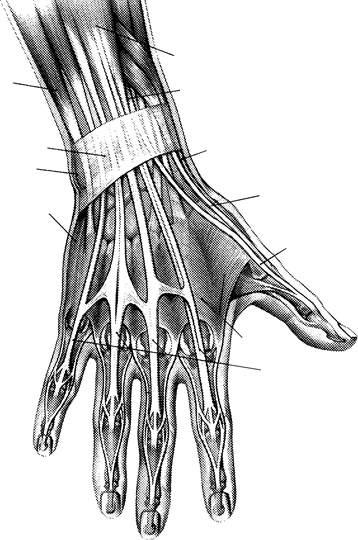
\includegraphics[width=4cm]{Handanatomy2}
\end{subfigure}
\begin{subfigure}
\includegraphics[width=4cm]{handanatomy}
\end{subfigure}
\caption{Hand Anatomy (taken from \cite{laviola1999survey})}
\label{fig:handAnatomyTotal}
\vspace{-15pt}
\end{figure}

\subsection{Deviation from Range of Rest Posture}

%rest on supports
\textbf{Range of Rest Posture (RRP)}, as defined by Apostolico et al. \cite{apostolico2014postural}, is a range of angles for an articular joint\footnote{The word ``articular joint" refers to joints in the human body.}, where the joint ``can be considered statistically in rest". The resulting relaxation of muscles and tendons creates maximum comfort in this particular joint. In our case, we considered the non-resting human hand to have a specific RRP for each finger joint, when the palm is facing downwards. Combining the RRPs of each finger joint for the entire hand results in a set of relaxed hand postures where comfort is maximized.

For articular joints perceived comfort decreases when deviating from the RRP and it minimizes at the bounds of the total range of motion. Applying this to the whole hand leads to the conclusion, that hand posture comfort can be evaluated by adding up the individual joint angle distances to the RRP~\cite{naddeo2015proposal}.

In our implementation the RRP was represented by a set of 50 relaxed hand postures recorded with the Leap. The metric \textbf{RRP(x)} was simply computed by calculating the minimum euclidean distance of a hand denoted as a multi-dimensional vector ``x" to the RRP set.
For simplicity we assumed comfort to linearly decrease with distance to the RRP in our metric.

\subsection{The Inter Finger Angles}

The hand has a very compact and highly connected system of muscles and tendons that limits the individual movement of fingers (Figure \ref{fig:handAnatomyTotal}).
Aside from the thumb, fingers share \textsl{most} of their flexor and extendor muscles. Despite that minor individual flexion and extension (Figure \ref{fig:hyperabduction}) of adjacent fingers is still possible due to finger tendons originating from different areas of the muscles. In the case of the EDC (\textit{Extensor digitorum communis}) the finger tendons are even interconnected on the back of the hand (Figure \ref{fig:handAnatomyTotal}). 

Based on this, we expect hand postures with high bending differences of adjacent fingers to cause stress of tendons and muscles, resulting in discomfort.

The \textbf{inter finger angle component} \textbf{IFA(x)} was computed by first adding up the flexion/extension angles of MCP (\textit{metacarpophalangeal}, PIP(\textit{proximal interphalangeal}) and DIP (\textit{distal interphalangeal}) joints (Figure \ref{fig:handAnatomyTotal}) for each finger. We then added up the differences in total bending of adjacent fingers (3 values). In order to compensate anatomical differences of the fingers, mostly affecting the ring finger, we added a ring finger bonus consisting of the difference of the ring finger's bending to both of its neighbors multiplied with an estimated weight coefficient. The importance of this differentiation can be seen when the fist is closed. Extending the ring finger from a closed fist is much harder than extending the index finger. 

\begin{figure}[b]
\centering
\vspace{-10pt}
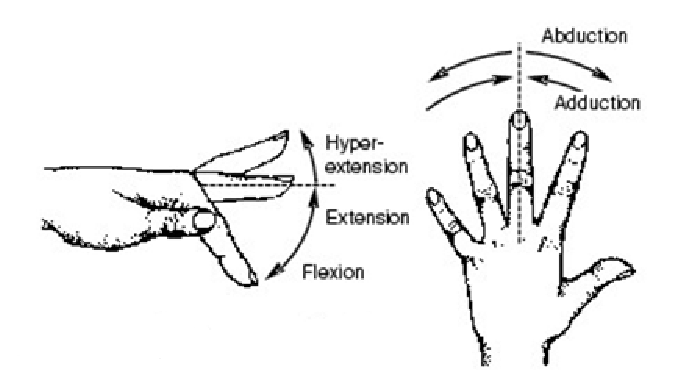
\includegraphics[width=7cm]{abduction}
\vspace{-10pt}
\caption{Hyperextension and Abduction (from \cite{laviola1999survey})}
\label{fig:hyperabduction}
\vspace{-10pt}
\end{figure}

\subsection{Finger Hyperextension}

As stated by LaViola, \textbf{hyperextension} (Figure \ref{fig:hyperabduction}) ``\textit{puts more strain on the }[MCP] \textit{joints and tendons than the hand is accustomed to}" and therefore causes discomfort \cite{laviola1999survey}.
Even though this might seem redundant to the deviation from RRP on first sight, hyperextension takes an increased toll as it causes considerably more discomfort, compared to a full flexion of the fingers and compared to what the deviation from RRP would suggest.

For the \textbf{hyper extension} component \textbf{HE(x)} we simply added up the flexion/extension angles of the fingers' MCPs that had a negative angle and were therefore hyperextended.

\subsection{Finger Abduction}

Finger \textbf{abduction} (Figure \ref{fig:hyperabduction})
also causes stress on the MCP joint, the abduction muscles and tendons involved.

Abduction was taken into consideration, analogue to the hyperextension, as full abduction creates substantially more discomfort than full adduction (Figure \ref{fig:hyperabduction}).

We computed the \textbf{abduction} component \textbf{FA(x)} by adding up the absolute abduction/adduction angle for the finger. This is possible as a fully adducted finger has an abduction angle of 0 in our model.


\subsection{Naive Metric}

After determining the single components, we designed our metric to be the added up component values \begin{math}(RRP, IFA, ...)\end{math} multiplied with weighting coefficients \begin{math}(c_{RRP(x)}, c_{IFA(x)}, ...)\end{math}. These weighting coefficients were estimated for the \textbf{naive metric.} 

	\[
	Naive(x) = c_{RRP}\cdot RRP(x) + c_{IFA}\cdot IFA(x)  +  c_{HE}\cdot HE(x)  +  c_{FA}\cdot FA(x)
	\]

We hypothesize that the resulting metric will correlate with user perception, having the value 0 as maximum for comfort and minimum for discomfort.

\subsection{Improved Metric}

Even though the naive metric contains the causes of comfort and discomfort, it still lacks deeper consideration for the anatomical differences between the fingers.
The concept of improvement extends the thought process already used for inter finger angles: instead of applying the metric to the whole hand, we consider the contributions from individual fingers and weight them with importance coefficients. 

	\[
	Improved(x) = c_{IFAindex}\cdot IFA(index(x))  +  c_{IFAmiddle}\cdot IFA(middle(x)) + ...
	\]

In our case we have five comfort values and a total of twelve discomfort values. 

However, the exact weighting coefficients are generally unknown and hard to estimate. To solve this problem, we reduced it to a curve fitting problem with 17 unknowns. We used data obtained from user studies to find the correct coefficients.

\section{Methodology}

For the collection of data, we created a test environment using \textbf{Unity 3D} with a total of two tasks. In the first task, the subject would be shown a randomly generated hand posture on screen. We used our naive metric to ensure a homogenous distribution of expected comfort and discomfort. The subject was asked to mimic the hand posture with his or her dominant hand and then rate the posture. As we did not expect the subjects to be familiar with current comfort and discomfort models, we asked them to rate hand postures on an intuitive scale ranging from 0 (very uncomfortable) to 10 (very comfortable). This was chosen over an ordinal Likert-like scale, because numerical values were needed for the metric's improvement and it's verification. The subject was told to rate the hand posture with 0 points if he or she was unable to reproduce it. Before beginning the evaluation, subjects were asked to form two hand postures so that they have a comfort/discomfort reference for the actual test. The first hand posture was a completely relaxed hand, the second hand posture was a randomly generated hand, that was challenging to mimic (such as the posture in figure \ref{fig:Robot}).

In the second task, the subjects were again given a randomly generated hand posture. Again the subject had to mimic the hand posture with his dominant hand and give it a rating from 0 to 10. After confirming his or her rating, the subject had to perform a target shooting task (Figure \ref{fig:participant}) with that specific posture. 
This specific task was chosen due to its similarity to real world tasks, where quick and precise spacial commands have to be issued.
We tracked the subject's hand using an \textbf{ART Tracking Device}. The software showed subjects a minimalistic representation of their hand position and indicated the forward direction of their hand with a ray. Subjects were seated, with the elbow rested on a table. They had to use this ray to aim down a total of 12 targets, appearing in random order, and shoot them, by pressing a button with the off-hand. By recording the hand posture before the trial using a Leap, and checking the hand posture during the test, we made sure that the subject would not break the posture. 

\begin{figure}[h]
\centering
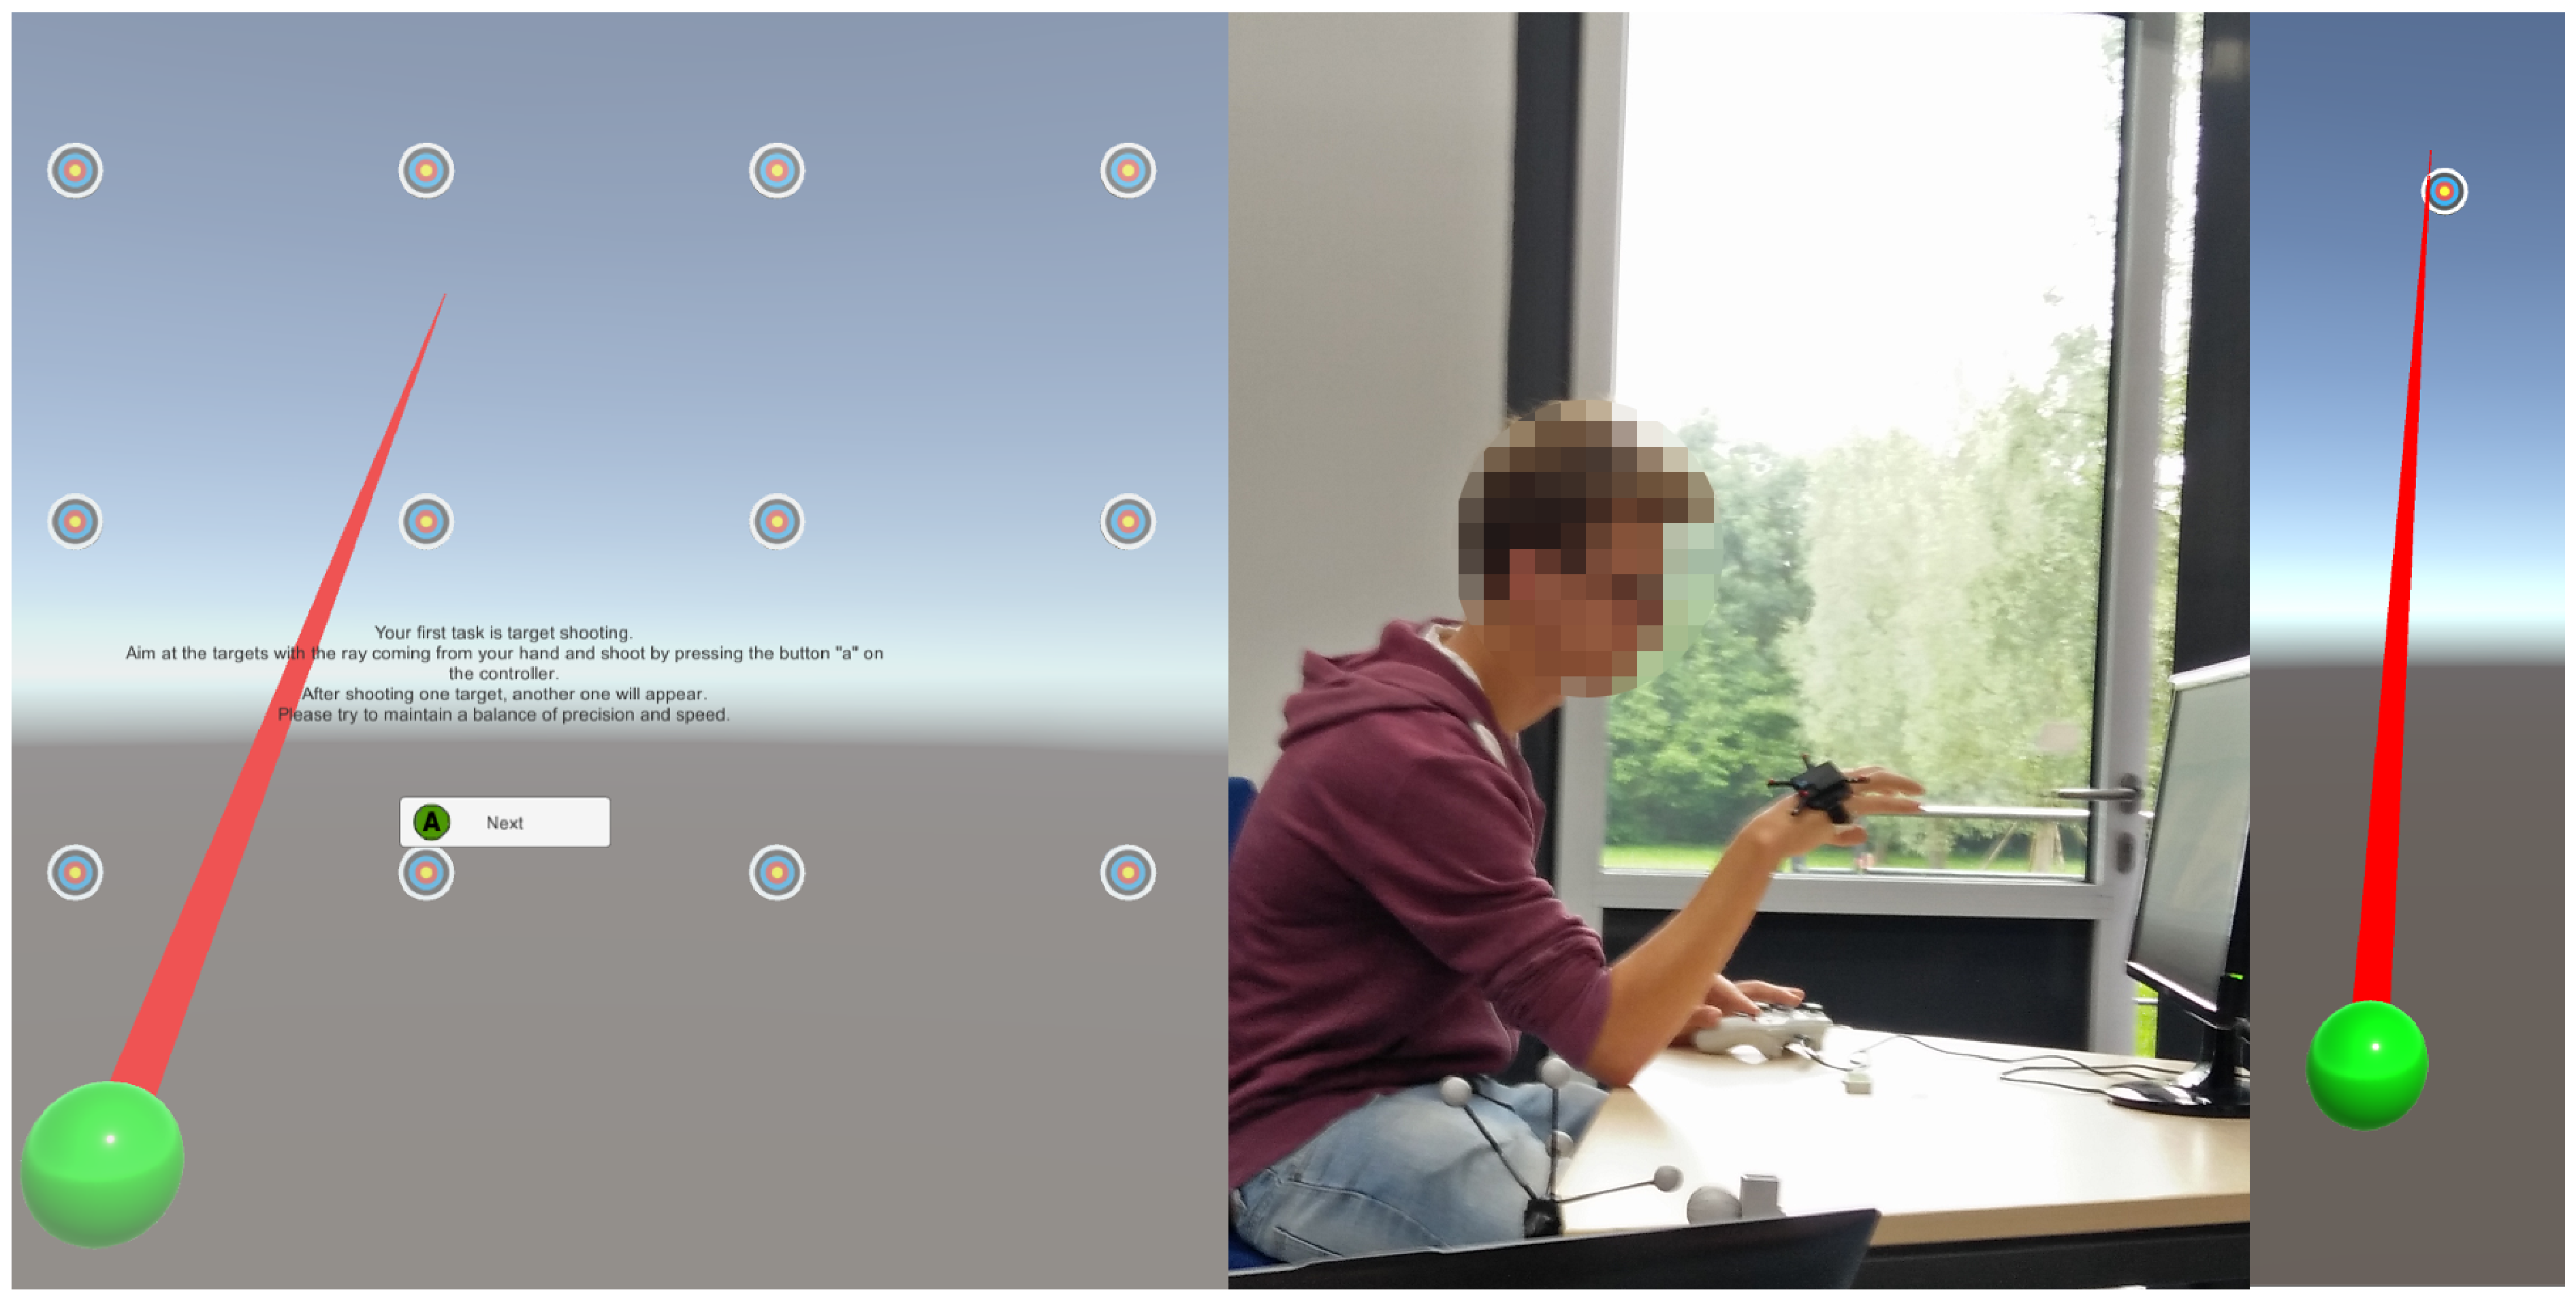
\includegraphics[width=8.45cm]{Participant}
\vspace{-20pt}
\caption{A Participant performing the Target Shooting (Best in Color)}
\label{fig:participant}
\vspace{-10pt}
\end{figure}

As a metric for performance, we measured the total time taken for the test. In order to have this affected by precision, we made the targets small and told the subjects to perform the test as quickly as possible.

We conducted a total of two user studies involving 21 participants, that resulted in 250 and 60 data sets for the metric and 35 data sets for the target shooting. Subjects were informed about the aim of the study as well as their specific objectives beforehand. 

Finding the best fitting coefficients can be reduced to a curve fitting problem. Therefore we used the least squares algorithm on the first 250 data sets to fit the comfort/discomfort values to the user ratings. Afterwards we tested our results against the remaining 60 data sets to validate them. For this, we decided to combine comfort and discomfort, as we expected both comfort and discomfort to affect performance.

\section{Results \& Discussion}

\begin{figure}[b]
\centering
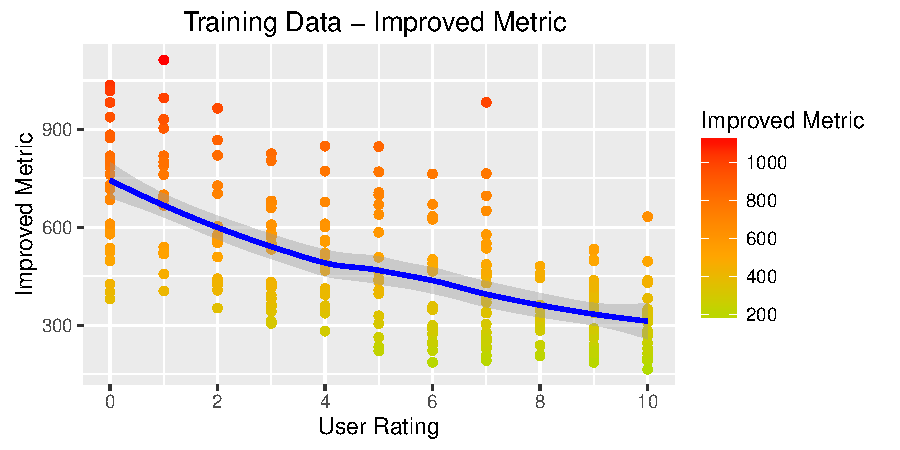
\includegraphics[width=8.45cm]{TrainingDataImproved.pdf}
\vspace{-20pt}
\caption{Improved Metric and User Rating in Training Data.\\
Correlation Coefficient: -0.645, p-value: < 2.2e-16}
\label{fig:trainingData}
\vspace{-10pt}
\end{figure}

For statistical analysis of the results, the Pearson correlation was used\footnote{The effect size is determined by the correlation coefficient. A correlation is significant if p < 0.01}.
The results are displayed in Figure \ref{fig:trainingData}-\ref{fig:targetShooting}, with the single samples shown as dots and the line indicating the smoothed conditional mean, calculated by the \texttt{geom\_smooth} function in R.
Unsurprisingly, the calculated values for the improved metric strongly affect the users comfort ratings, that were used to generate this metric (Figure \ref{fig:trainingData}). However, differences in anatomy and mindset of the participants and the limitation of hand posture ratings to 11 discrete steps introduced some noise to the data.

\begin{table}[t]
\centering
\caption{Weighting Coefficients of Improved Metric}
\label{tab:coeff}
\begin{tabular}{|c|l|l|l|l|l|} \hline
 &Thumb&Index&Middle&Ring&Pinky\\ \hline
RRP&0.631&-1.837&1.176&-3.021&1.288\\ \hline
IFA&-&0.547&0.216&1.670&-0.864\\ \hline
HE&-&-1.637&-2.685&10.401&-1.837\\ \hline
FA&-&-0.864&-3.857&0.0388&2.517\\
\hline\end{tabular}
\vspace{-10pt}
\end{table}

\begin{figure}[t]
\centering
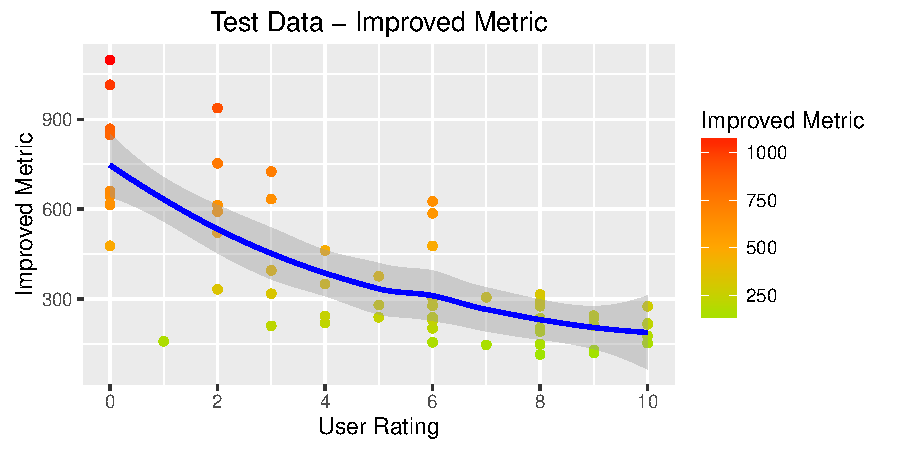
\includegraphics[width=8.45cm]{TestDataImproved.pdf}
\vspace{-20pt}
\caption{Improved Metric and User Rating in Test Data.\\
Correlation Coefficient: -0.748, p-value: 5.89e-12}
\vspace{-10pt}
\label{fig:testData}
\end{figure}

The computed weighting coefficients for the improved metric can be taken from Table \ref{tab:coeff}. Due to the small number of participants, the coefficients are very noisy and don't seem to make much sense. It can also be seen that the IFA coefficients are generally less noisy than those of HE or FA. This indicates, that the different components are perceived differently and that the metric has room for improvement.

Despite the noise, the created metric also holds its large effect on the user ratings even when applied to the test data (Figure \ref{fig:testData}). This shows, that the improved metric is a valid extrapolation of the training data and can be used to predict the perceived user comfort and discomfort of a certain hand posture.

\begin{figure}[b]
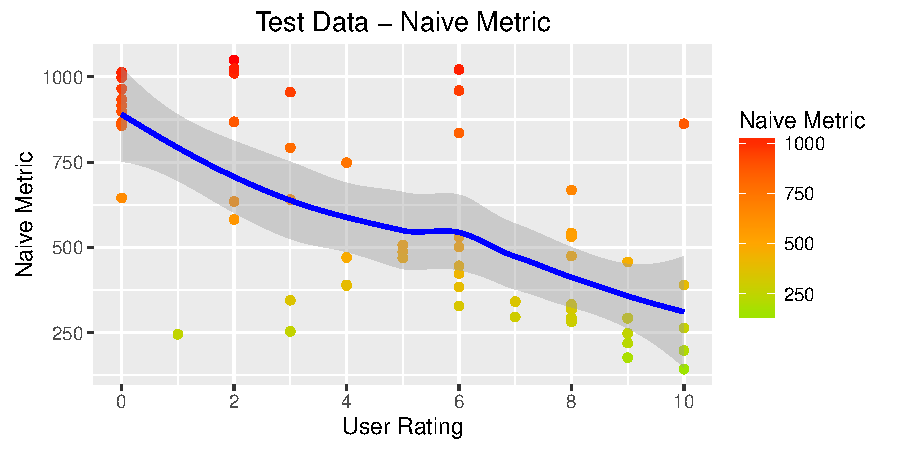
\includegraphics[width=8.45cm]{TestDataNaive.pdf}
\vspace{-20pt}
\caption{Naive Metric and User Rating in Test Data.\\
Correlation Coefficient: -0.665, p-value: 6.73e-9}
\label{fig:testDataNaive}
\vspace{-10pt}
\end{figure}

When looking at the naive metric, it can be seen that it predicts the user ratings in a similar way (Figure \ref{fig:testDataNaive}). However the improved metric creates a better prediction, as it reduces the metric values standard error.

\begin{figure}[h]
\centering
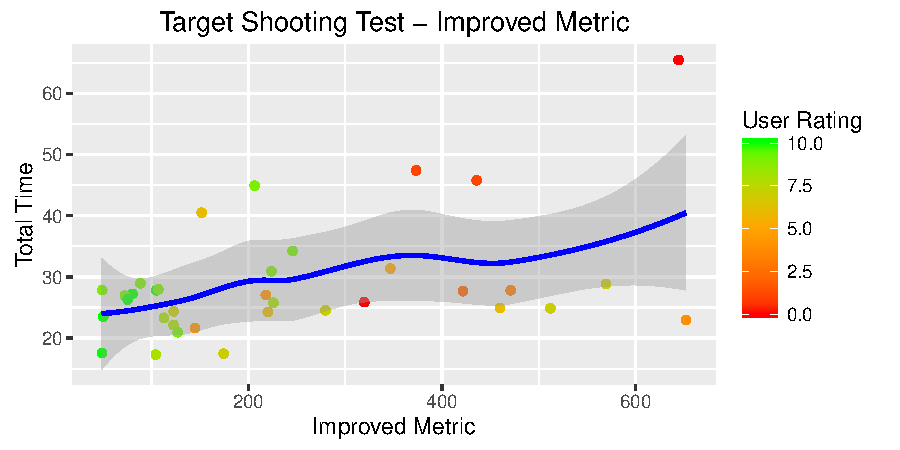
\includegraphics[width=8.45cm]{TargetShooting.pdf}
\vspace{-20pt}
\caption{Improved Metric Value and Total Task Time in Target Shooting.\\
Correlation Coefficient: -0.665, p-value: 6.73e-9}
\label{fig:targetShooting}
\vspace{-5pt}
\end{figure}

The results from the target shooting task (Figure \ref{fig:targetShooting}) shows that participants with harder hand postures generally took longer to finish. The large effect size is also confirmed by the Pearson correlation. This indicates that comfort and discomfort, as measured by our metric, significantly affect the performance and precision in context of hand postures. This strengthens the conclusion of Short et al.~\cite{short1999precision}, that more comfortable postures generally create greater accuracy. However, the credibility of our results is limited by the relatively small number of participants. Further work is required before strong conclusions can be made.

\section{Conclusion \& Future Work}
The main goal of this paper was to create a basic metric for quick and objective evaluation of hand posture comfort and discomfort. Furthermore we demonstrated the metric's relevance for design of hand postures, by proving its influence on precision and performance in a 3D pointing task. For the creation of the metrics we applied knowledge of hand anatomy and state of the art comfort and discomfort models and used data from a user study to improve it. Results from the testing user study suggest the improved metric to be a valid extrapolation of the training data. In addition, the outcome of a small target shooting test indicate the existence of a correlation between comfort/discomfort and precision/performance, as already suggested for different contexts in other papers.

This work was only a first step for exploring hand posture comfort and discomfort. The metric created is still primitive and has some room for improvement. Furthermore only the short-term effects of comfort and discomfort combined were studied. An important next step would be to investigate the long- and short-term effects of comfort and discomfort separately in order to create more sophisticated models and metrics.
%\end{document}  % This is where a 'short' article might terminate

%
% The following two commands are all you need in the
% initial runs of your .tex file to
% produce the bibliography for the citations in your paper.
\bibliographystyle{abbrv}
\bibliography{handComfort}  % sigproc.bib is the name of the Bibliography in this case
% You must have a proper ".bib" file
%  and remember to run:
% latex bibtex latex latex
% to resolve all references
%
% ACM needs 'a single self-contained file'!
%
%APPENDICES are optional
%\balancecolumns

%\balancecolumns % GM June 2007
% That's all folks!
\end{document}
